% --- Template for thesis / report with tktltiki2 class ---

\documentclass[finnish]{../tktltiki2}

% tktltiki2 automatically loads babel, so you can simply
% give the language parameter (e.g. finnish, swedish, english, british) as
% a parameter for the class: \documentclass[finnish]{tktltiki2}.
% The information on title and abstract is generated automatically depending on
% the language, see below if you need to change any of these manually.
% 
% Class options:
% - grading                 -- Print labels for grading information on the front page.
% - disablelastpagecounter  -- Disables the automatic generation of page number information
%                              in the abstract. See also \numberofpagesinformation{} command below.
%
% The class also respects the following options of article class:
%   10pt, 11pt, 12pt, final, draft, oneside, twoside,
%   openright, openany, onecolumn, twocolumn, leqno, fleqn
%
% The default font size is 11pt. The paper size used is A4, other sizes are not supported.
%
% rubber: module pdftex

% --- General packages ---

\usepackage[utf8]{inputenc}
\usepackage{lmodern}
\usepackage{microtype}
\usepackage{amsfonts,amsmath,amssymb,amsthm,booktabs,color,enumitem,graphicx}
\usepackage[pdftex,hidelinks]{hyperref}

% Automatically set the PDF metadata fields
\makeatletter
\AtBeginDocument{\hypersetup{pdftitle = {\@title}, pdfauthor = {\@author}}}
\makeatother

% --- Language-related settings ---
%
% these should be modified according to your language

% babelbib for non-english bibliography using bibtex
\usepackage[fixlanguage]{babelbib}
\selectbiblanguage{finnish}

% add bibliography to the table of contents
\usepackage[nottoc]{tocbibind}
% tocbibind renames the bibliography, use the following to change it back
\settocbibname{Lähteet}

% --- Theorem environment definitions ---

\newtheorem{lau}{Lause}
\newtheorem{lem}[lau]{Lemma}
\newtheorem{kor}[lau]{Korollaari}

\theoremstyle{definition}
\newtheorem{maar}[lau]{Määritelmä}
\newtheorem{ong}{Ongelma}
\newtheorem{alg}[lau]{Algoritmi}
\newtheorem{esim}[lau]{Esimerkki}

\theoremstyle{remark}
\newtheorem*{huom}{Huomautus}


% --- tktltiki2 options ---
%
% The following commands define the information used to generate title and
% abstract pages. The following entries should be always specified:

\title{Ohjelmistoala ja ryhmätyöskentely}
\author{Kenny Heinonen}
\date{\today}
\level{Aine}
\abstract{Tiivistelmä.}

% The following can be used to specify keywords and classification of the paper:

\keywords{avainsana 1, avainsana 2, avainsana 3}
\classification{} % classification according to ACM Computing Classification System (http://www.acm.org/about/class/)
                  % This is probably mostly relevant for computer scientists

% If the automatic page number counting is not working as desired in your case,
% uncomment the following to manually set the number of pages displayed in the abstract page:
%
% \numberofpagesinformation{16 sivua + 10 sivua liitteissä}
%
% If you are not a computer scientist, you will want to uncomment the following by hand and specify
% your department, faculty and subject by hand:
%
% \faculty{Matemaattis-luonnontieteellinen}
% \department{Tietojenkäsittelytieteen laitos}
% \subject{Tietojenkäsittelytiede}
%
% If you are not from the University of Helsinki, then you will most likely want to set these also:
%
% \university{Helsingin Yliopisto}
% \universitylong{HELSINGIN YLIOPISTO --- HELSINGFORS UNIVERSITET --- UNIVERSITY OF HELSINKI} % displayed on the top of the abstract page
% \city{Helsinki}
%


\begin{document}

% --- Front matter ---

\maketitle        % title page
%\makeabstract     % abstract page

\tableofcontents  % table of contents
\newpage          % clear page after the table of contents


% --- Main matter ---

\section{Johdanto}

Ohjelmistojen kehityksen perustana on ryhmätyöskentely, koska projektien
kasvava kompleksisuus ja laajuus tekee niiden toteuttamisen yksilölle
vaikeaksi~\cite{5593527}.
Ohjelmistoalalla tarvitaan monenlaisia teknisiä taitoja, jotta projekteissa saadaan toteutettua kaikki kehityksen vaiheet 
kattavasti. Nämä ohjelmistokehityksen vaiheet voidaan jakaa karkeasti 
vaatimusmäärittelyyn, suunnitteluun, toteutukseen, testaukseen ja 
ylläpitoon~\cite{Capretz:2010:MSS:1726559.1726574}\footnote{Capretz puhuu järjestelmäanalyysista, joka on sidoksissa vaatimusmäärittelyyn. Tässä tekstissä käsitellään järjestelmäanalyysin sijaan vaatimusmäärittelyä.}. Sen lisäksi, että 
eri vaiheet vaativat eri taitoja, myös yksittäinen vaihe kysyy laajaa 
osaamista. Tämän seurauksena tulee tarve koota joukko osaavia ihmisiä 
toteuttamaan yhteistyössä kaikki kehityksen vaiheet. Onkin hyvin 
tavanomaista, että ohjelmistoprojektit toteutetaan ryhmätyönä.\\

Ryhmätyö vaatii teknisten taitojen lisäksi yhteistyö- ja kommunikointitaitoja, koska
se vaikuttaa ryhmän suorituskykyyn~\cite{Hall:2007:CNT:1235000.1235043}. Ryhmätyön merkitys ollaan
tunnettu jo kauan ja sitä painotetaan yhä enemmän tietojenkäsittelytieteiden opetusohjelmissa~\cite{Cushing:2003:TBP:948785.948797,5593527,1158709,Pieterse:2012:PPS:2157136.2157218}.
Useat prosessimallit jopa sanelevat miten ryhmätyöskentely tapahtuu, jotta kehitys sujuisi luontevammin ja tuotteliaammin.
Kehittäjien välinen yhteistyö riippuu myös yksilöstä ja siitä miten heidän persoonallisuudet ja
luonteenpiirteet sopivat yhteen~\cite{Acuna:2008:ESP:1414004.1414056,Hall:2007:CNT:1235000.1235043}. Tarkoituksena on tarkastella ketteriä menetelmiä ja tutkia miten muutamat esimerkkimenetelmät
määräävät ohjelmistokehityksen luonteesta painottaen ryhmän sisäistä toimintaa. Lisäksi kuvataan
millainen on ideaali ryhmän jäsen ja
millä luonteenpiirteillä on vahvimmat positiiviset vaikutukset kehityksen eri vaiheisiin. \\

\section{Ketterät menetelmät ja ryhmätyöskentely}

% Write some science here.

%Ryhmätyöskentelyä voi tehdä monin tavoin. On esimerkiksi tilanteita, joissa ryhmät sijaitsevat samoissa oloissa, mutta työskentelevät silti täysin erillään toisistaan.Tämän seurauksena kommunikointi kärsii ja voi olla epäsäännöllistä.
Ketterät menetelmät pohjautuvat 12 ketterän 
kehityksen periaatteeseen~\cite{AgileManifesto}. Ryhmätyöskentelyllä 
ja yhteistyöllä on ketterissä
menetelmissä suuri painoarvo. Esimerkiksi eräs periaate on, että 
\emph{"parhaat arkkitehtuurit, vaatimukset ja suunnitelmat syntyvät 
itseorganisoituvissa
tiimeissä"}. Tämä tarkoittaa pitkälti sitä, että tiimit työskentelevät 
yhdessä päättäen asioista ilman, että kukaan ulkopuolinen tulee
kertomaan heille mitä tehdä ja miten. Toisin sanoen tiimiä johtaa tiimi itse, 
tiimillä ei ole johtajaa tai projektipäällikköä. Periaatteissa 
painotetaan
myös informaation välittämistä kasvokkain käytävillä keskusteluilla. 
Ryhmillä tulisi olla yhteiset työtilat, jolloin tämä periaate 
toteutuisi.
Kasvokkainen kommunikointi virtaviivaistaa tiedon kulkua ja pienentää 
väärinkäsitysten mahdollisuutta.\\

Ketterissä menetelmissä toimivan ohjelmiston tuottaminen säännöllisin 
väliajoin on tärkeää ja sillä halutaan pitää asiakas tyytyväisenä.
Ketterät menetelmät perustuvatkin iteratiiviseen ja inkrementaaliseen kehitysmalliin, jossa tuotetta kehitetään lyhyissä kehityssykleissä osa kerrallaan~\cite{Cockburn:2008}. Kehitysmallissa ohjelmiston toteuttamiseen tarvittava työ pilkotaan osiin, jotka aikataulutetaan niin, että kukin osa kehitetään ajan myötä valmiiksi lyhyissä kehityssykleissä. Tuotetta rakennetaan valmiiksi säännöllisin väliajoin, jolloin asiakas näkee kehityksen ja voi antaa palautetta kertoen meneekö kehitys oikeaa suuntaa kohti.\\

Seuraavissa osioissa tutustumme kahteen tunnettuun
ketterään menetelmään nimeltään \emph{Scrum} ja \emph{Extreme Programming}~\cite{ScrumFinnishGuide,Scrumprimer,ScrumHandBook,Beck:2004:EPE:1076267}. Muitakin menetelmiä toki on, mutta ne jätetään käsittelemättä. Osioissa kerrotaan millaisen prosessin nämä menetelmät
määrittelevät projektin kehitykselle ja miten niissä otetaan ryhmätyöskentely ja kommunikointi huomioon.

\subsection{Extreme Programming}

\emph{Extreme Programming} (XP) on ketterä menetelmä, jonka tunnettu 
ohjelmistokehittäjä Kent Beck on luonut. XP keskittyy asiakkaan tyytyväiseen. XP:n tarkoituksena on tuottaa 
asiakkaalle mahdollisimman paljon arvoa mahdollisimman tehokkaasti ja nopeasti.
XP:ssä kehitys tapahtuu lyhyissä, 1-4 viikon iteraatioissa, jolloin vaatimusten 
muutoksiin on helpompi varautua, kun tavoitteet on asetettu 
lähitulevaisuuteen. XP painottaa ketterien menetelmien tapaan kommunikointia ja ryhmätyötä.

\subsubsection{Kommunikointi}

Kasvokkaista ja usein tapahtuvaa kommunikointia painotetaan järjestämällä tiimin jäsenet yhteiseen tilaan. Tämän lisäksi projektia varten on hankittu vähintään yksi paikan päällä oleva asiakas, joka on osana kehitystiimiä nähdäkseen projektin edistymisen. Paikan päällä olevan asiakkaan kanssa keskustellaan kehityksen jokaisesta vaiheesta ja hän päättää tuotteen vaatimuksista ja niiden priorisoinnista. Asiakkaan läsnäolo on suuri etu, sillä tiimi voi kysyä häneltä hetkessä esimerkiksi jonkin toteutettavan vaatimuksen yksityiskohdista ja asiakas vastaavasti voi antaa heti palautetta työstä. Ryhmän sisäinen kommunikointi on myös suuressa osassa sillä hyvät ratkaisut saadaan useimmiten yhteistyön tuloksena. Kommunikoinnin ja yhteistyön merkitystä kuvastaa esimerkiksi \emph{pariohjelmointi} (pair 
programming), joka on yksi XP:n keskeisimpiä käytänteitä.
Tutustutaan pariohjelmointiin tarkemmin.

\subsubsection{Pariohjelmointi}

Pariohjelmoinnissa kaksi henkilöä ohjelmoivat pareittain, jakaen saman 
tietokoneen~\cite{Shore:2007:AAD:1407480}. Henkilöt eivät kuitenkaan ohjelmoi samaan aikaan, vaan 
heille on 
nimetty kaksi roolia: toinen on \emph{ajaja} (the driver), ja toinen 
\emph{navigoija} (the navigator). Ajajan tehtävänä on 
yksinkertaisesti 
kirjoittaa koodia. Navigoijan tehtävänä on analysoida jatkuvasti 
kirjoitettua koodia ja kertoa ajajalle mitä tehtäviä heidän tulee 
milloinkin 
toteuttaa. Näin ajaja voi keskittyä pelkästään ohjelmointiin. Sovituin 
väliajoin henkilöt vaihtavat rooleja. Pariohjelmointi voidaan nähdä 
ryhmätyöskentelynä --- kaksi ihmistä suorittavat yhteistä tehtävää 
saavuttaakseen saman päämäärän.\\

Pariohjelmointi korostaa yhteistyötä ja kommunikointia. Tästä on monia 
hyötyjä, jotka tekevät hyvää sekä ryhmän jäsenille, ryhmälle että 
projektille~\cite{Begel:2008:PPW:1414004.1414026}. Tarkastellaan näitä 
hyötyjä seuraavaksi. 

\begin{itemize}

\item {\bf Koodin laatu}

Kun kaksi henkilöä pariohjelmoivat ja ratkaisevat samaa ongelmaa, 
lopputulos on usein tehokkaampi verrattuna siihen, että yksi henkilö 
tekisi kaiken. Parit pystyvät helposti keskustelemaan keskenään siitä 
mitä heidän tulisi seuraavaksi tehdä ja he voivat jakaa ideoita 
saadakseen koodista laadukkaamman tai ratkaistakseen jonkin ongelman. 
Sivustakatsojana navigoija pystyy tekemään tärkeitä huomioita ja 
pohtimaan kuinka koodista saataisiin laadukkaampi, kun taas ajaja voi 
keskittyä ohjelmoimiseen. Navigoija tekee ajoittain ehdotuksia 
ajajalle, jolla koodista saataisiin parempaa.
Pariohjelmoinnin ansiosta tapahtuva laajamittaisempi koodin 
katselmointi vähentää virheiden määrää. Vaihtoehtoisesti
niitä ei edes synny, kun parit keskenään kommunikoivat miettien hyviä 
ratkaisuja.

Pariohjelmointi parantaa keskittymiskykyä. Toisen henkilön 
läsnäolo estää herkemmin yksilöä laiskottelemasta tai rikkomaan XP:n
vaalimia käytänteitä, kuten TDD:tä. Käytänteiden noudattaminen taas 
johtaa parempaan koodin laatuun ja toteutukseen.

\item {\bf Oppiminen}

Kun henkilöt "pariutuvat"~toistensa kanssa, niin osaaminen 
leviää kehittäjien kesken. Monet tykkäävät neuvoa toisiaan ja ryhmän 
jäsenillä
on eri taitoja ja tietämystä asioista. Esimerkiksi ryhmän jäsenet, 
jotka pääsevät heitä taitavampien ihmisten pareiksi voivat oppia
paljon uusia tekniikoita. Parhaimmassa tapauksessa koko ryhmän sisällä 
kaikki voivat oppia toisiltaan jotakin.
Oppimiseen sisältyy, että ymmärrys kehitettävästä ohjelmasta 
parantuu. Kun henkilöt vaihtavat
pareja eri ihmisten kanssa, he pääsevät näkemään erilaisia 
kehityksessä olevia ohjelman osia. Samalla he osallistuvat tämän 
yhden osan
kehitykseen, jolloin ymmärrys koko projektista kasvaa korkeammalle 
tasolle.\\

Tästä voidaan päätellä, että pariohjelmointi on suuressa roolissa 
XP:ssä ja ryhmän jäsenien keskinäisellä vuorovaikutuksella on suuri 
hyöty projektin laadun kannalta. Kaikkien näiden pariohjelmoinnin 
hyvien puolien yhteisenä tekijänä on, että parit kommunikoivat 
toistensa kanssa. Ilman keskinäistä vuorovaikutusta ei voi odottaa, 
että edellä mainitut asiat toteutuisivat. Pariohjelmointi kuitenkin 
rohkaisee kehittäjiä puhumaan toisilleen, joten tästä ei pitäisi olla 
huolta~\cite{Zarb:2012:UCW:2384716.2384738}.

\end{itemize}

\subsubsection{Julkaisusuunnittelun kokous}

Kun asiakas on tehnyt listan vaatimuksia, joita kehitettävän järjestelmän pitää sisältää, aloitetaan XP:n prosessi \emph{julkaisusuunnittelun kokouksella} (release planning meeting),
jossa on tarkoituksena tehdä \emph{julkaisusuunnitelma} (release plan). XP:ssä on tapana iteraatioiden lopuksi julkaista uusin, toimiva versio asiakkaiden käyttöön. Julkaisusuunnitelma määrittelee, mitkä vaatimukset toteutetaan missäkin iteraatiossa ja siten ovat valmiina iteraation lopuksi tehtävässä julkaisussa. Näille vaatimuksille määritellään päivämäärät.\\

Kokouksessa kehitystiimin tehtävänä on arvioida kuinka paljon yksittäinen vaatimus vie työaikaa. Estimointien perusteella asiakas
tekee päätök\-sen vaatimusten prioriteeteista. Tämän jälkeen tiimin jäsenet
yhdessä asiakkaan kanssa sijoittavat vaatimukset tietyille iteraatioille toteutettaviksi.

\subsubsection{Iteraatiosuunnittelun kokous}

Ennen kuin varsinainen iteraatio alkaa, jossa itse tuotteen tiettyjen toiminnallisuuksien
kehitys tapahtuu, järjestetään \emph{iteraatiosuunnittelun kokous} (iteration planning meeting), jossa tehdään \emph{iteraatiosuunnitelma} (iteration plan). Iteraatiosuunnittelun tavoitteena on päättää mitä iteraation aikana tehdään, joka kirjataan iteraatiosuunnitelmaan.\\

Suunnittelun alussa asiakas valitsee julkaisusuunnitelmasta korkeimman prioriteetin omaavat vaatimukset alkavaan iteraatioon. Kehittäjät pilkkovat nämä vaatimukset pieniksi, toteutettaviksi tehtäviksi. Tämän jälkeen kehittäjät päättävät ketkä toteuttavat minkäkin tehtävän ja he estimoivat tehtäviin kuluvan työmäärän. Lopuksi vaatimukset, tehtävät ja niiden estimaatit kirjataan iteraatiosuunnitelmaan.

\subsubsection{Iteraatio}

Iteraatiosuunnittelun ja onnistuneen suunnitelman tekemisen jälkeen voidaan aloittaa itse iteraatio. Iteraatio kestää 1-4 viikkoa, jonka aikana iteraatiosuunnitelmaan kirjatut vaatimukset ja niihin liittyvät tehtävät pitää toteuttaa. Kehitystyö tapahtuu pariohjelmoiden, jonka
merkitystä ryhmätyöskentelyyn tarkasteltiin luvussa 2.1.2. Iteraatioon liittyy päivittäinen palaveri, jossa ryhmän jäsenet raportoivat toisilleen mitä saivat viime palaverin jälkeen aikaan, mitä aikovat saada aikaan ennen seuraavaa palaveria ja onko heidän etenemisessään ongelmia. Näin tiimin jäsenet ovat jatkuvasti tietoisia
muiden jäsenten sekä koko tiimin tilanteesta. Kuten edellä on mainittu, iteraation aikana on vähintään yksi asiakas läsnä joka päivä, jonka kanssa voi puhua ongelmatilanteissa toteutettavien vaatimusten yksityiskohdista ja neuvotella kehityksestä.\\

Iteraation lopuksi suoritetaan \emph{hyväksymätestaus} (acceptance testing), jossa testataan iteraation aikana toteutettuja vaatimuksia ja varmistutaan siitä, että ne toimivat oikein. Asiakas on määritellyt tarkemmin mitä skenaarioita testien tulisi testata. Jos yksittäinen vaatimus läpäisee kaikki siihen kohdistuvat testit, on vaatimus toteutettu valmiiksi. Asiakas itse tarkistaa testitulokset ja päättää niiden perusteella onko viimeisin versio tuotteesta julkaisukelpoinen. Jos testauksen aikana löytyy ohjelmointivirheitä, ne kirjataan ylös ja korjataan seuraavan iteraation aikana.\\

Ketteränä menetelmänä XP on iteratiivinen, joten kun yksi iteraatio on loppunut, aloitetaan edellä mainittu prosessi uudestaan alkaen julkaisusuunnittelun kokouksella. Näin XP:n prosessia jatketaan, kunnes tuote on valmis. XP painottaa hyvin paljon asiakkaan kanssa kommunikointia ja läsnäoloa, jotta kehityksessä ei päädytä sivuraiteille. Asiakas on osana ryhmää ja hänen kanssaan tapahtuva kommunikointi ja yhteistyö vaikuttaa suuresti projektin onnistumiseen yhdessä ryhmän sisäisen kommunikoinnin kanssa.

\subsection{Scrum}

\begin{figure}[ht]
     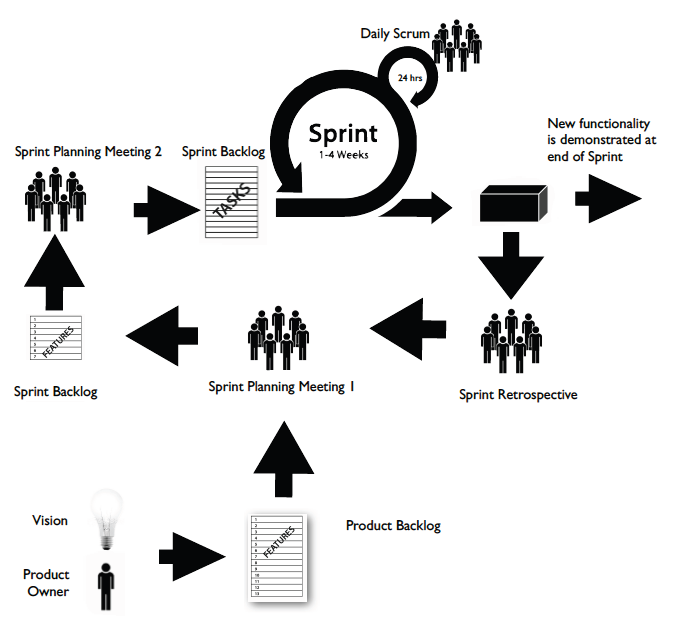
\includegraphics{scrum.png}
     \caption{Scrumin prosessi~\cite{Scrumprimer}}\label{scrumprocess}
\end{figure}

Scrum on prosessimalli, joka painottaa tiimien yhteistyötä projektin 
kehityksessä~\cite{ScrumORG}. Scrum, kuten XP, on myös iteratiivinen 
ja inkrementaalinen menetelmä.
Kehitys tapahtuu lyhyissä 1-4 viikon sykleissä, 
\emph{"sprinteissä"}, joissa toteutetaan kehitettävää tuotetta tietyt 
toiminnallisuudet kerrallaan. Lyhyet kehityssyklit sallivat tiimien 
mukautuvan asiakkaalta saatavaan palautteeseen ja vaatimusten 
muutoksiin. Näin tuotteeseen voidaan tehdä ajoissa
muutoksia ilman suuria kuluja ja tuote "hioutuu"~yhä lähemmäs sitä 
mitä asiakas sen haluaa olevan. Scrum tekee projektin kehityksestä
monivaiheisen, kuten kuvassa \ref{scrumprocess} näkyy. Nämä vaiheet tullaan käsittelemään myöhemmin. Seuraavissa osioissa kerrotaan millainen Scrum-tiimi
on ja millainen projektin elinkaari on Scrumissa.

\subsubsection{Tiimi}

Scrumissa tiimit koostuvat \emph{monitaitoisista} (cross-functional) 
jäsenistä, joilta löytyy tarpeellinen tekninen osaaminen, jota 
vaaditaan
tuotteen toteuttamiseksi. Tiimillä ei ole johtajaa tai 
projektipäällikköä, jotka määräisivät tiimin tekemisistä. Sen sijaan 
tiimi itse
saa päättää tavoitteet joka sprintille ja sen miten nämä tavoitteet 
saavutetaan. Toisin sanoen tiimi on \emph{itseorganisoituva}
(self-organizing). Tämä on Scrumille olennaista ja siitä näkee 
kuinka suuressa arvossa tiimin jäsenten välistä yhteistyötä 
pidetään~\cite{ScrumHandBook}.

\subsubsection{Scrumin aloitus}

Scrumin ensimmäinen askel on luoda visio tuotteen vaatimista
ei-toiminnalli\-sista ja toiminnallisista vaatimuksista. Vaatimukset
kootaan listaksi, jota kutsutaan \emph{tuotteen kehitysjonoksi} (product backlog)~\cite{ScrumFinnishGuide}. Kehitysjono on priorisoitu siten, että tärkeimmät vaatimukset ovat kehitysjonon kärjessä. Kehitysjono on jatkuvan muutoksen alaisena: uusia vaatimuksia
voi tulla lisää asiakkaan toimesta, tarpeettomia vaatimuksia karsitaan ja olemassaolevia muokataan tai tarkennetaan. Edellä mainitut tehtävät
ovat niin kutsutun \emph{tuoteomistajan} (product owner) vastuulla,
joka on yksittäinen henkilö ja pitää huolen tuotteen arvon ja kehitystiimin työn arvon maksimoimisesta. Tuoteomistaja voi kuitenkin pyytää kehitystiimiä auttamaan edellä mainituissa tehtävissä.

\subsubsection{Sprintin suunnittelupalaveri}

Jokaisen sprintin aluksi järjestetään kokous, jota kutsutaan \emph{sprintin suunnittelupalaveriksi} (sprint planning meeting)~\cite{ScrumHandBook}. Palaveri on kaksiosainen.
Ensimmäisessä osassa tuoteomistaja ja kehitystiimi neuvottelevat
siitä mitkä vaatimukset tiimin tulisi toteuttaa alkavassa
sprintissä. Päätösvastuu on kuitenkin tiimin jäsenillä.\\

Toisessa osassa tiimi valitsee toteutettavat vaatimukset, jotka
he sitoutuvat tekemään sprintin loppuun mennessä. Vaatimukset
valitaan aina kehitysjonon kärjestä ylhäältä alas järjestyksessä.
Kun vaatimukset on valittu, ne hajotetaan pienemmiksi, teknisiksi
tehtäviksi. Nämä tehtävät kirjataan \emph{sprintin tehtävälistaan} (sprint backlog) aika-arvioineen, mitä tiimi käyttää hyödykseen sprintin ajan. Tiimi saa itse valita toteutettavat vaatimukset alkavalle sprintille ja suunnitella miten ne toteutetaan.

\subsubsection{Scrumin päiväpalaveri}

Kun sprintti alkaa, sen aikana harjoitetaan erästä Scrumin käytäntöä:
\emph{päiväpalaveria} (daily Scrum). Tämä on lyhyt, noin 15 minuuttia kestävä kokoontuminen joka päivä samaan aikaan, johon
kaikki tiimin jäsenet osallistuvat. Jokainen tiimin jäsen saa
mahdollisuuden raportoida kolme asiaa muille tiimin jäsenille:
mitä henkilö on saanut aikaan viime tapaamisen jälkeen, mitä henkilö
aikoo saada aikaan ennen seuraavaa tapaamista ja onko mitään
esteitä työn etenemiselle? Näin tiimin jäsenet säännöllisesti tietävät
kuinka muiden työ edistyy ja palaverin jälkeen mahdollisia raportoituja
ongelmia voidaan yhdessä ratkoa. Huomionarvoista on, että on yleisesti
suositeltua, että päiväpalaveriin ei osallistu esimiehiä tai muita
ulkopuolisia henkilöitä~\cite{ScrumHandBook}. Jos näin käy, on riski,
että henkilöt tuntevat olevansa tarkkailun alaisena, joka voi
tuottaa heille paineita oman edistymisen tai ongelmien raportoinnista.

\subsubsection{Sprintin katselmointi}

Sprintin lopussa järjestetään \emph{sprintin katselmointi} (sprint review), jossa tiimi esittelee sprintin aikana toteuttamiaan
vaatimuksia tuoteomistajalle ja asiakkaalle. Asiakas ja tuoteomistaja
tietävät näin miten projekti on edistynyt ja tiimi vastaavasti saa
arvokasta palautetta kyseisiltä henkilöiltä. Tämä on motivoivaa
kaikille osapuolille. Annettu palaute kirjataan mahdollisina muutoksina
vaatimuksiin tai uusina vaatimuksina tuotteen kehitysjonoon.

\subsubsection{Sprintin retrospektiivi}

Viimeisenä asiana sprintin lopuksi järjestetään \emph{sprintin retrospektiivi}
(sprint retrospective), jossa tiimi keskustelee kuinka heidän
oma työprosessinsa sujui sprintin aikana~\cite{Scrumprimer}. Käytännössä jäsenet
keskustelevat yhdessä mikä sprintissä sujui hyvin ja missä
asioissa pitäisi parantaa. Jäsenien antama palaute ja kritiikki
voi esimerkiksi kohdistua yksittäisen jäsenen työskentelytapoihin.
Jos mahdollisia ongelmakohtia on, tiimin tulisi yhdessä päättää
miten nämä ongelmat ratkaistaan. Retrospektiivi on tärkeä vaihe
ryhmätyöskentelyn kannalta sillä se on Scrumin pääasiallisin
mekanismi tuoda tiimin ongelmat näkyville ja ratkaista ne siten,
että ryhmän työskentely vahvistuu ja paranee.\\

Kun nämä kaikki edellä mainitut vaiheet on käyty läpi, alkaa uusi
sprintti. Käytännössä aloitetaan uusi sykli aloittaen
sprintin suunnittelupalaverista. Tätä periaatteessa jatketaan
niin kauan, kunnes tuote on valmis eli asiakkaan kaikki vaatimukset
on toteutettu. Kuten monista asioista kävi ilmi, kehitystiimin jäsenillä on paljon valtaa sen suhteen mitä he tekevät ja miten he
sen tekevät. Suunnittelutyö ja toteutus on asia, jonka tiimin
jäsenten pitää yhteisymmärryksessä päättää kommunikoiden toistensa kanssa.

\section{Persoonallisuuden vaikutus}

Kehitystiimit koostuvat erilaisista ihmisistä ja useissa tutkimuksissa on huomattu, että tietyt
luonteenpiirteet ja persoonallisuustyypit vaikuttavat positiivisesti tiimin suorituskykyyn sekä
projektin onnistumiseen~\cite{Acuna:2008:ESP:1414004.1414056,Gorla:2004:WWB:990680.990684,Capretz:2003:PTS:766407.766410,Capretz:2010:MSS:1726559.1726574}. Sen lisäksi, että tiimien olisi hyvä koostua monitaitoisista
jäsenistä, moninaiset persoonallisuustyypit tiimin sisällä ovat hyväksi
projektille. Esimerkiksi suurempia ratkaisuja mietittäessä harvoin hyväksytään
ensimmäinen ehdotus, joka esitetään, vaan puntaroidaan monen ehdotuksen
välillä arvioiden niiden hyviä ja huonoja puolia. Myös yksilön oma
tekninen osaaminen vaikuttaa ratkaisun miettimiseen. Eri tavalla ajattelevat ihmiset kykenevät tuomaan joukon
eri näkökulmia tuotetta kehitettäessä, joka johtaa parempiin ratkaisuihin.\\

Edellä mainitun lisäksi henkilön persoonallisuus vaikuttaa
siihen
kuinka mieluista kyseisen henkilön kanssa on työskennellä,
miten henkilö lähestyy annettua tehtävää ja minkälaisiin tehtäviin
hän soveltuu parhaiten~\cite{Begel:2008:PPW:1414004.1414026,Capretz:2010:MSS:1726559.1726574}. Eräs tapa mitata henkilön persoonallisuutta on käyttää Myers-Briggsin tyyppi-indikaattoria.
Seuraavissa osioissa tarkastellaan millaisia piirteitä hyvällä
ohjelmistokehittäjällä on ja mitkä erilaiset persoonallisuustyypit
sopivat parhaiten projektien eri kehitysvaiheisiin. Ennen tätä kuitenkin kerrotaan millainen Myers-Briggsin tyyppi-indikaattori on, jonka avulla pohjustetaan tulevia osioita.

\subsection{Myers-Briggsin tyyppi-indikaattori}

Persoonallisuustyyppejä määriteltäessä käytetään apuna
Myers-Briggsin tyyppi-indikaattoria, joka jakaa ihmisen persoonallisuuden neljään eri osioon: sosiaaliseen vuorovaikutukseen, tiedonkeruuseen, päätöksentekoon ja elämän\-tyyliin~\cite{Capretz:2003:PTS:766407.766410,Capretz:2010:MSS:1726559.1726574,DaCunha:2007:PMA:1230819.1241672}. Joka osiossa on
kaksi eri luonteenpiirrettä. Kussakin osiossa jokainen ihminen kallistuu enemmän toiseen piirteeseen kuin toiseen eli Myers-Briggsin
tyyppi-indikaattorilla saadaan yksittäiselle henkilölle näistä osioista neljä luonteenpiirrettä, jotka määrittävät hänen persoonallisuuden. Yhteensä
persoonallisuustyyppejä on $2^4$ = 16 erilaista.

\begin{enumerate}

\item Sosiaalinen vuorovaikutus: Ekstrovertti (E) --- Introvertti (I)

Ekstrovertit ovat sosiaalisia, ulospäinsuuntautuneita ja nauttivat
muiden ihmisten seurasta. Introvertit sen sijaan ovat sisäänpäinkääntyneitä, hiljaisia, varautuneita ja ovat mieluummin omissa oloissaan.

\item Tiedonkeruu: Tosiasiallinen (S) --- Intuitiivinen (N)

Tosiasialliset ihmiset etsivät yksityiskohtaista tietoa ja tunnettuja
tosiasioita. He uskovat enemmän konkreettisiin asioihin, jotka
voivat itse omin aistein todistaa. Intuitiiviset etsivät asioille
yhteyksiä teoreettisemman ja abstraktisemmankin tiedon pohjalta ja
he miettivät eri asioista aiheutuvia mahdollisuuksia.

\item Päätöksenteko: Ajatteleva (T) --- Tunteva (F)

Ajattelevat perustavat päätöksensä miettimällä tarkasti päätöksen syitä, seurauksia ja loogisuutta. He perustavat päätöksensä puhtaaseen järjen käyttöön. Tuntevilla on taipumusta tehdä päätös
henkilökohtaisten arvojen perusteella ja sen mukaan miten päätös
vaikuttaa muihin ihmisiin. Päätöksenteko-ulottuvuus vaikuttaa siihen minkälaisista tehtävistä
henkilö kiinnostuu ja kuinka tyytyväinen hän on niihin.

\item Elämäntyyli: Järjestelmällinen (J) --- Spontaani (P)

Järjestelmälliset ihmiset ovat sananmukaisesti järjestelmällisiä
ja täsmäl\-lisiä. He pitävät aikamääreistä kiinni ja suunnittelevat
asioita etukäteen. Spontaanit taas ovat joustavia ja elävät
hetkessä välittämättä suunnitelmallisuudesta ja järjestelmällisyydestä.
Elämäntyyli-ulottuvuus vaikuttaa henkilön työskentelytapoihin.

\end{enumerate}

\subsection{Hyvän ohjelmistokehittäjän piirteet}

Usein todetaan, että hyvälle ohjelmistokehittäjälle on aina tilaa ohjelmistoalalla.
Siinä missä tekninen osaaminen ja hyvä tietämys asioista on
tärkeää, myös ihmistaidot ja kommunikointi on alkanut keräämään
huomiota alalla~\cite{Hall:2007:CNT:1235000.1235043}. Esimerkiksi
pariohjelmoinnissa työskentely vaatii kommunikointia ja sitä, että
tulee toisten ihmisten kanssa toimeen. Seuraavaksi tarkastellaan ohjelmistokehittäjän piirteitä, jotka tekevät henkilöstä mieluisen työkumppanin teknisten taitojen lisäksi.
Tutkimuksissa
on haastateltu ohjelmistoalan ammattilaisia ja kysytty heiltä mitkä
piirteet ja asiat tekevät hyvän ohjelmistokehittäjän~\cite{Acuna:2008:ESP:1414004.1414056,Begel:2008:PPW:1414004.1414026,Hall:2007:CNT:1235000.1235043}. Haastattelujen perusteella seuraavat piirteet ovat tärkeimpiä:

\begin{itemize}

\item {\bf Joustava \& mukautuva}

Joustava henkilö on avaramielinen. Henkilö kuuntelee mielellään muiden
ideoita ja kykenee katsomaan asioita eri näkökulmista sen sijaan, että
puolustelisi vain omaa kantaansa. Lisäksi hän on halukas yhteistyöhön
ja pystyy mukautumaan eri työtapoihin.

\item {\bf Hyvät kommunikointitaidot}

Ohjelmiston kehittäminen vaatii paljon ryhmätyöskentelyä ja
kommunikointia tiimin jäsenten kesken. Hyvä kommunikoija kykenee
kuuntelemaan muiden ideoita, ilmaisee omat mielipiteensä selkeästi ja uskaltaa
kysyä apua, jos hänellä on ongelmia. Kun tiimi koostuu jäsenistä,
jotka kommunikoivat usein ja hyvin, se vaikuttaa positiivisesti
ilmapiiriin ja työn laatuun. Esimerkiksi kommunikoinnin myötä
tieto leviää tiimin jäsenten kesken, joka kasvattaa kaikkien osaamista.

\item {\bf Älykäs}

Ohjelmistokehitys on pohjimmiltaan teknistä työtä, joten
ihmistaitojen lisäksi myös älykkyys on erittäin tärkeä piirre.
Älykkyydellä tarkoitetaan tässä tapauksessa ohjelmistokehittäjää, jolla on hyvä tekninen osaaminen ja hän on nopea
ajatuksissaan. Henkilön ongelmanratkaisutaidot ovat erinomaiset
ja hän kykenee ajattelemaan asioita abstraktilla tasolla sekä ottaa
vastuuta työstään.

\item {\bf Mukava}

Mukava ohjelmistokehittäjä on sosiaalinen ja hänen kanssaan on
helppo työskennellä. Hänellä on huumorintajua ja sopivaa
tilannetajua eli esimerkiksi pystyy huomauttamaan virheistä ilman,
että toinen pahastuu. Lyhyesti sanottuna kyseisen henkilön kanssa
on hauska työskennellä.

Muita mainittuja piirteitä olivat muun muassa, että ohjelmistokehittäjä
on tietäväinen, innovatiivinen, itsenäinen, kykenee keskittymään työhönsä, ja noudattaa käytettyä prosessia.

\end{itemize}

\subsection{Persoonallisuustyypit eri kehityksen vaiheissa}

Ohjelmiston kehitys on monivaiheinen prosessi ja perinteisessä ohjelmistotuotannossa se on
jaettu vaatimusmäärittelyyn, suunnitteluun, toteutukseen, testaukseen
ja ylläpitoon. Nämä eri vaiheet vaativat erilaisia teknisiä taitoja,
jotta saadaan paras mahdollinen lopputulos. Kuitenkin teknisen
osaamisen lisäksi myös persoonallisuustyyppi vaikuttaa siihen kuinka
hyvin henkilö suoriutuu tietyistä tehtävistä tai kuinka hyvin hän
soveltuu niihin~\cite{Capretz:2010:MSS:1726559.1726574}. Kun luonteiltaan oikeanlaiset henkilöt valitaan suorittamaan
näitä tiettyjä kehityksen vaiheita, tuloksena on parempi lopputulos
projektin kannalta.\\

Seuraavaksi käydään edellä mainitut kehityksen vaiheet läpi yksi kerrallaan
ja tarkastellaan millaiset ohjelmistokehittäjät sopivat
parhaiten mihinkin vaiheeseen. Oletetaan, että kehittäjillä on
hyvä tekninen osaaminen kaikissa vaiheissa, jolloin tarkastelu
voidaan rajoittaa ainoastaan siihen kuinka hyvin he persoonallisuustyypeiltään soveltuvat suorittamaan tiettyjä
kehityksen vaiheita.

\subsubsection{Vaatimusmäärittely}

Perinteisesti ohjelmistotuotanto alkaa vaatimusmäärittelyllä~\cite{SWEBOK:409902,Sommerville:2005:IRE:1042197.1042341}. Tämän vaiheen tavoitteena on selvittää mitä vaatimuksia
tuotteella eli valmiilla ohjelmalla on. Vaatimuksilla voidaan tarkoittaa toiminnallisia vaatimuksia eli
mitä ohjelma tekee tai mitä sillä pystytään tekemään, tai ei-toiminnallisia vaatimuksia eli esimerkiksi millä kielellä
ohjelma kirjoitetaan, kuinka käytettävä tai tehokas sen tulee olla ja niin edelleen.\\

Vaatimusmäärittely tehdään usein asiakkaan kanssa, jolla on etukäteen jonkinlainen kokonaiskuva valmiista ohjelmasta.
Kehittäjien tehtävänä on haastatella asiakasta saadakseen selville millaisesta ohjelmasta on kyse ja mitä sen tulisi tehdä.
Vaatimusmäärittelyssä tulee kartoittaa ensinnäkin keitä ovat ohjelman käyttäjät ja millaisia käyttötilanteita
käyttäjillä on ohjelmaan liittyen. Yhteistyössä asiakkaan kanssa saadaan lopuksi lista vaatimuksia toteutettavalle ohjelmalle,
jotka seuraavaksi analysoidaan. Analysoinnilla tutkitaan ovatko vaatimukset tarpeeksi kattavat eli määrittävätkö ne asiakkaan
haluaman tuotteen sekä tarkistetaan, että vaatimukset eivät ole ristiriidassa toistensa kanssa. Jos vaatimukset vaikuttavat
kattavilta ja ristiriidattomilta, niin lopuksi vielä varmistetaan asiakkaalta, että vaatimukset ovat hänen mieleensä ja
edustavat sitä mielikuvaa tuotteesta, joka hänellä on.
Lopuksi vaatimukset dokumentoidaan, jotta kehittäjät tietävät ja muistavat jatkossakin mitä heidän tulee toteuttaa sekä testata.\\

Capretz ja Ahmed ovat tutkineet millainen kehittäjä soveltuu
parhaiten järjestelmäanalyysiin, joka on sidoksissa vaatimusmäärittelyyn~\cite{Capretz:2010:MSS:1726559.1726574}.
Järjestelmä\-analyysiin tarvitaan kehittäjiä, jotka ymmärtävät asiakkaan tarpeet ja käsittävät mitkä ovat ohjelman keskeisimmät toiminnot.
Järjestelmäanalyysi vaatii paljon kommunikointia asiakkaan kanssa,
joten ekstrovertit (E) soveltuvat tähän hyvin, koska he ovat parempia
puhumaan ja saamaan asiakkaasta vastauksia irti toisin kuin introvertit (I), jotka eivät ole yhtä hyviä ilmaisemaan asioita selkeästi. 
Kehittäjän tulee myös osata asettumaan käyttäjän rooliin ja miettimään
käyttäjän tarpeita. Tähän tarpeeseen on tuntevat (F) ihmiset hyviä. Vaatimusmäärittelyssä keskustellaan samaan tapaan asiakkaan kanssa, joissa tämän kaltaiset henkilöt ovat tarpeellisia. Optimaalisinta olisi määrätä vaatimusmäärittelyyn kehittäjiä, jotka ovat sekä ekstrovertteja että tuntevia (EF).\\

Gorlan ja Lamin mielipiteet eroavat edellä mainitusta~\cite{Gorla:2004:WWB:990680.990684}. Heidän mukaan ajattelevat (T) kehittäjät ovat tuntevia (F) parempia tässä työssä, jos kyse on pienestä tiimistä. Pienemmissä tiimeissä vaatimusten määrittelyn lisäksi kehittäjä voi joutua tekemään paljon muutakin, kuten suunnittelua ja ohjelmointia, jolloin analyyttinen ajattelutapa on parempi.

\subsubsection{Suunnittelu}

Suunnittelu on prosessi, jossa määritellään ohjelman arkkitehtuuri, komponentit, rajapinnat ja muut ohjelmaan liittyvät asiat~\cite{SWEBOK:409902}.
Suunnittelussa hahmotellaan vaatimusten perusteella mistä komponenteista ja pienemmistä osasista järjestelmä koostuu ja mitkä ovat niiden tehtävät. Suunnittelussa mietitään miten järjestelmän eri osat ovat vuorovaikutuksessa toistensa kanssa, millaiset rajapinnat niillä on ja mitä palveluita ne tarvitsevat muilta järjestelmän osilta.
Tarkoituksena on luoda ohjelmasta malli, joka toteuttaa kirjatut vaatimukset, ja jonka voi muuttaa ohjelmakoodiksi.\\

Suunnittelu on luovaa ja tutkivaa työtä, jossa suunnittelija miettii mitkä ovat järjestelmän avainkomponentit, ja hahmottelee parhaita ratkaisuja erilaisten käyttötilanteiden avulla. Suunnittelijalla tulisi olla kokonaiskuva järjestelmästä ja kyky erotella relevantit asiat annetusta datasta, kuten vaatimuksista. Tämä vaatii intuitiota.
Suunnittelijoiden tulisi siis olla intuitiivisia (N), koska tällaiset henkilöt ovat luovia ja innostuvat uusien asioiden luomisesta ja kokeilevat erilaisista asioista tapahtuvien mahdollisuuksien yhdistelyä. Hyvän tuloksen saamiseksi tarvitaan ongelmanratkaisutaitoja, joita ajattelevilla (T) on. On suositeltavaa, että suunnittelija on sekä intuitiivinen ja ajatteleva (NT)~\cite{Capretz:2010:MSS:1726559.1726574}.

\subsubsection{Toteutus}

Kun suunnittelu on ohi, siirrytään toteutukseen~\cite{SWEBOK:409902}. Suunnitteluvaiheessa ohjelmasta ollaan luotu jonkinlainen malli siitä millaisista komponenteista se koostuu
ja mitkä ovat eri komponenttien tehtävät, voidaan ryhtyä toteuttamaan tätä mallia. Käytännössä tämä tarkoittaa
mallin muuntamista koodiksi ja siten konkreettiseksi ohjelmaksi.\\

Toteutus on suurimmaksi osaksi ohjelmointia, johon liittyy suunnittelua ja testausta. Ohjelmoijan tulee tunnistaa ohjelman
osille tärkeät muuttujat, rakenteet ja tietorakenteet. Ohjelmoijan
tulee luonnollisesti hallita ohjelmointikieli, jolla ohjelma kirjoitetaan. Siinä missä ohjelmalle tehty malli voi olla hyvinkin korkeatasoinen, koodin kirjoittaminen vaatii paneutumista yksityiskohtiin ja mallin sekä vaatimusten muuntaminen suoraviivaiseksi koodiksi vaatii loogista ajattelutapaa. Ajatteleva (T)
henkilö soveltuu loogiseen ajatteluun paremmin kuin tunteva (F). Lisäksi yksityiskohtiin ja faktatietoihin paneutuminen on tosiasiallisen (S) ihmisen aluetta enemmän kuin intuitiivisen (N). Vaikka aiemmin on todettu kehityksen vaativan ryhmätyötä ja kommunikointia, Capretz ja Ahmed näkevät ohjelmoinnin teknisenä työnä, joka loppupeleissä vaatii itsenäistä työskentelyä ja keskittymiskykyä enemmän kuin ryhmätyöskentelyä. Täten introvertit (I) sopivat ohjelmoijiksi ekstrovertteja (E) paremmin. Ihanteellinen yhdistelmä ohjelmoijalle olisi, että hän on introvertti, tosiasiallinen ja ajatteleva (IST). Tätä väitettä tukee se, että monien tutkimusten mukaan useimmat ohjelmistokehittäjät ovat persoonallisuustyyppiä ISTJ~\cite{Capretz:2003:PTS:766407.766410,Capretz:2010:MSS:1726559.1726574}.\\

Gorlan ja Lamin havainnot poikkeavat ideaalista ohjelmoijasta~\cite{Gorla:2004:WWB:990680.990684}, kun kyse on pienistä tiimeistä. Tiimin suorituskyky on parempi, jos ohjelmoijat ovat ekstrovertteja (E). Pienissä tiimeissä ohjelmoijien pitää kommunikoida useiden osapuolten kanssa, kuten esimerkiksi muiden tiimin jäsenten kanssa. Lisäksi pienissä tiimeissä ohjelmoija voi joutua tekemään monia muitakin tehtäviä kuin vain ohjelmointia, kuten ohjelman suunnittelua ja kommunikointia asiakkaan tai käyttäjien kanssa. Tällöin ekstroverttius on eduksi.
\looseness=-1

\subsubsection{Testaus}

Testausvaiheessa on tarkoituksena tehdä testejä, joilla varmistetaan ohjelman toimivuus~\cite{SWEBOK:409902}. Vaatimukset ovat ensisijaisia
testauskohteita eli testien avulla tarkistetaan, että ohjelmalle asetetut vaatimukset, jotka ovat toteutettu, toimivat
moitteettomasti. Testauksella pyritään myös löytämään ohjelmasta mahdollisimman paljon virheitä tekemällä testitilanteita, joissa yritetään
tehdä jotain luvatonta toimintaa, jota ohjelman ei tulisi sallia. Esimerkiksi, jos ohjelma on yksinkertainen laskin,
joka pyytää syöttämään yhteenlaskua varten kaksi lukua ja käyttäjä yrittää syöttää kirjaimista koostuvan merkkijonon, ohjelman
tulee osata varautua tähän ilman, että se hajoaa.\\

Testausta on monenlaista, joita ovat muun muassa yksikkötestaus,
integrointitestaus ja järjestelmätestaus~\cite{Capretz:2010:MSS:1726559.1726574}.
Yksikkötestauksessa testataan ohjelman sisältämiä komponentteja, luokkia
ja metodeita yksilöllisesti. Integraatiotestauksessa varmistetaan, että nämä komponentit, luokat ja metodit toimivat niiden ollessa keskinäisessä vuorovaikutuksessa toistensa kanssa, pyytäen ja tarjoten palveluita toisilleen. Järjestelmätestauksessa ohjelmaa testataan sen rajapinnan eli useimmiten käyttöliittymän kautta. Järjestelmätestaus liittyy vahvasti vaatimuksiin, jotka määrittävät, että järjestelmällä pitäisi pystyä tekemään jotain ja järjestelmän tulisi vastata tähän toimintoon vaatimusten mukaisesti.\\

Testaukseen on monenlaisia strategioita, jotka noudattavat järjestelmälli\-siä lähestymistapoja. Testaus vaatii paneutumista yksityiskohtiin, jotta testaaja varmasti tarkistaa, että pienimmätkin ohjelman osat toimivat oikein. Tarkkuus ja järjestelmällisyys ovat
haluttavia ominaisuuksia testaajalle, joita tosiasialliset (S) ja järjestelmälliset (J) henkilöt edustavat. Menestyvät testaajat olisivat sekä tosiasiallisia että järjestelmällisiä (SJ)~\cite{Capretz:2010:MSS:1726559.1726574}.

\subsubsection{Ylläpito}

Ennen ylläpitoa ohjelma on jo julkaistu kohderyhmän käyttöön valmiina tuotteena, joka toteuttaa vaatimukset~\cite{SWEBOK:409902}. Ylläpidon
tarkoituksena on parannella tai muokata ohjelmaa, jolla tarkoitetaan lähinnä ohjelmointivirheiden
korjaamista ja optimointia. Ylläpidossa saatetaan lisätä myös aivan uusia toiminnallisuuksia
ohjelmaan. Kaiken tämän tarkoituksena on pidentää ohjelman käyttöikää ja varmistaa käyttäjien
tyytyväisyys.\\

Ohjelman ylläpitäminen ja parantelu sopii tosiasiallisille (S) kehittäjille, koska he suosivat tuttujen tehtävien tekoa, jotka eivät vaadi uusien asioiden kokeilua. Intuitiiviset (N) sen sijaan haluavat kokeilla jotain uutta ja luultavasti tylsistyisivät ylläpitoon, jossa tehdään jonkinlaisia parannuksia ja pieniä ohjelmointivirheiden korjauksia. Tosiasialliset suosivat töitä, joissa aiemmin opitun tiedon käyttö on riittävää tehtävän suorittamiseen sen sijaan, että tulisi keksiä uusia ratkaisuja. He myös osaavat keskittyä yksityiskohtiin ja haluavat tietää miten asiat toimivat, joten heillä olisi hyvä kokonaiskuva järjestelmästä, jota ylläpitäminen vaatii. Spontaanit (P) sopeutuvat muutoksiin, jolloin heitä ei haittaisi järjestelmän jatkuva muokkaaminen. Siten tosiasialliset ja spontaanit kehittäjät ovat hyviä ylläpitäjiä (SP)~\cite{Capretz:2010:MSS:1726559.1726574}.\\

Edellä mainitut vaiheet ovat kaikki oleellisia ketterissä menetelmissä. Ketterät menetelmät perustuvat iteratiiviseen ja inkrementaaliseen kehitysmalliin, jonka ideana on tehdä ohjelmisto sykleissä, joissa ohjelmistosta tuotetaan vain osa. Tämä osa tuotetaan valmiiksi niin, että sykli sisältää vaatimusmäärittelyn, suunnittelun, toteutuksen, testauksen ja ylläpidon. Käytännössä tämä tarkoittaa, että yhden syklin aikana sama tiimi työstää yhdessä näitä vaiheita eli tiimin jäseniä ei eroteta ottamaan vastuuta vain tietystä vaiheesta. Kuten on todettu, monipuolinen tiimi eri persoonallisuuksilla täytettynä tuottaa paljon eri näkökulmia ja ratkaisuja. Persoonallisuutta katsottaessa yksittäinen henkilö saattaa olla toista henkilöä parempi tietyssä kehityksen vaiheessa, joten ketterissä menetelmissä on hyvä olla tiimi, jonka jäsenet ovat erilaisia luonteiltaan.

\subsection{Huonon ohjelmistokehittäjän piirteet}

Ohjelmistoalalla on väistämättä huonojakin ohjelmistokehittäjiä, jotka
tekevät yhteistyöstä epämiellyttävää. Hallin ja kumppaneiden haastatteluissa kysyttiin millaisia ovat huonot kehittäjät~\cite{Hall:2007:CNT:1235000.1235043}. Tuloksena oli, että huono ohjelmistokehittäjä on tekniseltä osaamiseltaan heikko ja hänellä on huonot kommunikointitaidot. Huonoilla kommunikointitaidoilla haastateltavat tarkoittivat seuraavia asioita:

\begin{enumerate}

\item Ei raportoi ongelmista.
\item Haluton kuuntelemaan muiden ideoita.
\item Itsepäinen.
\item Ei kunnioita ylempiarvoisia.

\end{enumerate}

Kun tähän lisätään luvun 3.2 hyvien piirteiden vastakohtia, on huono kehittäjä huumorintajuton, ei ota työstään vastuuta ja hänellä on vaikeuksia omaksua uusia työtapoja tai rooleja. Tekniseltä osaamiseltaan kehittäjän ongelmanratkaisutaidot ovat heikot eikä hänellä ole kykyä ajatella asioita abstraktisti.\\

Mainitsemisen arvoisia ovat Pietersen ja kumppaneiden kertomista yksittäisen henkilön osallistumisen tasoista ryhmätyös\-kentelyssä~\cite{Pieterse:2012:PPS:2157136.2157218}. Tasoja on neljä, joista
kaksi eivät ole ryhmälle hyväksi:

\begin{itemize}

\item {\bf Diligent isolate}

Yksilö luottaa vain itseensä tehtäviä suoritettaessa eikä halua muilta apua. Hän näkee
muut ryhmän jäsenet tehottomina ja kyvyttöminä suorittamaan tehtävää ja tuloksena voi olla, että
hän lannistaa muiden ryhmän jäsenien motivaatiota.

\item {\bf Social loafer}

Yksilön panos ryhmätyöhön on vähäisempi kuin muiden ryhmän jäsenten ja hän
tekee vähemmän kuin mitä häneltä odotetaan. Joskus hän saattaa ottaa kunnian muiden
tekemästä työstä.

\end{itemize}

Pietersen ja kumppaneiden tekemässä ryhmätyöhön liittyvässä kokeilussa havaittiin, että ryhmistä löytyi jäseniä, joiden osallistumisen taso vastasi edellä mainittuja.

\section{Ryhmätyötaitojen parantaminen}

Hyvät ryhmätyö- ja kommunikointitaidot eivät ole itsestäänselvyys. Itse asiassa monesti on todettu, että
tietojenkäsittelytieteen opiskelijoiden ryhmätyö- ja kommunikointitaidot ovat puutteelliset johtuen siitä, että opetuksessa näitä taitoja ei ole huomioitu tarpeeksi~\cite{Cushing:2003:TBP:948785.948797,5593527,Waite:2004:SCV:1028174.971308}. Ryhmätyöskentelyn merkitys on huomattu ja
opetusohjelmiin on lisätty enemmän ryhmä- ja projektitöitä, mutta varsinaisia kommunikointitaitoja ei opiskelijoille opeteta, jotka auttaisivat
heitä menestymään paremmin näissä töissä. Tämän seurauksena opiskelijat eivät välttämättä osaa toimia ryhmässä ja kokemus jää epämiellyttäväksi, joka vaikuttaa negatiivisesti asenteisiin ryhmätyöskentelyä kohtaan~\cite{1158709}.
Luvussa 3.4 todettiin huonon ohjelmistokehittäjän piirteitä. Henkilö, joka täyttää osankin kyseisistä piirteistä, ei ole houkutteleva ryhmän jäsen. Kuitenkin haastattelujen perusteella tällaisia ihmisiä löytyy ohjelmistoalalta.\\

Puutteelliset ja jopa huonot ryhmätyötaidot huomioon ottaen on tarve menetelmille, joilla parantaa yksilön ryhmätyötaitoja.
Seuraavaksi tarkastellaan erilaisia menetelmiä, joilla
kehittää yksilöiden kommunikointi- ja ryhmätyötaitoja, jotta he pystyisivät toimimaan tehokkaasti ryhmänä. Menetelmät on
kehitetty suurimmaksi osaksi opetuskäyttöön opiskelijoille,
jotka eivät ole vielä työelämässä.

\subsection{Kevyet menetelmät}

\subsubsection{Vuorovaikutteinen luokkahuone}

\emph{Vuorovaikutteinen luokkahuone} (the conversational classroom) on menetelmä, jolla demonstroidaan opiskelijoille yhteistyön etuja~\cite{Waite:2004:SCV:1028174.971308}. Tässä menetelmässä opettaja panee aluille keskustelua kurssimateriaaliin liittyen sen sijaan, että pitäisi luennon kurssimateriaalista itse. Näin opettaja kannustaa opiskelijoita keskustelemaan keskenään materiaalista. Opiskelijat oppivat toisiltaan asioita ja se
aktivoi heitä verrattuna perinteiseen luentoon, jossa opiskelijan
rooli on olla passiivinen kuuntelija. Waiten ja kumppaneiden mukaan hänen yliopistossaan vuorovaikutteinen luokkahuone on ollut onnistunut kokeilu, joka on parantanut opiskelijoiden tehokkuutta ja yhteistyötaitoja.

\subsubsection{Tarkkailija-kommunikoija-rakentaja}

\emph{Tarkkailija-kommunikoija-rakentaja} (observer-communicator-builder) on kevyt harjoitus, jossa
opiskelijat jaetaan ryhmiin tarkoituksena kehittää
kommunikointia~\cite{Cushing:2003:TBP:948785.948797}. Yksittäinen
ryhmä sisältää kolme henkilöä, joilla jokaisella on yksi seuraavista
rooleista, jotka ovat menetelmän nimen mukaisesti tarkkailija, kommunikoija tai rakentaja.\\

Harjoituksen ideana on tuottaa rakennelma, jonka mallin saa selittää vain sanallisesti. Henkilöt järjestetään
kolmeen eri alueeseen siten, että tarkkailija ja rakentaja ovat
toisistaan erillään eivätkä pysty viestimään toisilleen muuten
kuin kommunikoijan kautta. Tarkkailijalla on malli rakennelmasta,
jonka rakentajan tulee tehdä. Tarkkailija kertoo rakennusohjeita
sanallisesti kommunikoijalle, joka välittää ohjeet eteenpäin rakentajalle. Harjoitus järjestetään siten, että jokainen ryhmän
jäsen pääsee kokeilemaan kaikkia rooleja. Iteraatioiden kautta
ryhmän jäsenien kommunikointitaidot kehittyvät ja he vähitellen päätyvät samalle aaltopituudelle siten, että jäsenet ymmärtävät ja tulkitsevat toistensa viestit samalla tavalla.

\subsection{Suuret menetelmät}

\subsubsection{Projektilähtöinen oppiminen}

\emph{Projektilähtöinen oppiminen} (Project-based learning) on menetelmä, jonka voi sisällyttää opetukseen ja sen perustana on
antaa opiskelijoille monimutkainen ongelma, jonka opiskelijat
ratkaisevat ryhmätyön muodossa.
Huang Jun artikkelissa \emph{"Improving undergraduates' teamwork skills by adapting project-based
learning methodology"}~esittää kuinka projektilähtöisen oppimismenetelmän voi
sisällyttää tietojenkäsittelytieteen opetukseen~\cite{5593527}.
Menetelmän ensimmäinen askel on
pitää johdantokurssi tietojenkäsittelystä ja alan tutkimuksesta.
Kurssin myötä opiskelijat saavat tarvittavaa tietämystä ryhmätyössä tehtävää projektia
varten. Johdantokurssin lisäksi opiskelijat tutustutetaan erilaisiin algoritmeihin,
suunnittelumalleihin ja näiden toteuttamiseen ohjelmointikielellä. Ohjelmointitaidon
opettelu on avuksi projektia varten.\\

Menetelmän toinen askel on, että opiskelijat muodostavat ryhmät itse perustuen opiskelijoiden
taustoihin tietojenkäsittelytieteen suhteen ja sen mukaan minkä tyyppisiä projekteja kukin
opiskelija haluaa toteuttaa. Ryhmät valitsevat projektin aiheen omin päin, joka on avainaskel
kehittämään opiskelijoiden luovuutta ja innovaatiota. Projektien tavoitteet määritellään
löyhästi, jolloin opiskelijoilla on vapaus keksiä useita eri ratkaisuja. Opettajat auttavat
ryhmiä alkuun kehittelemällä opiskelijoiden kanssa alustavan suunnitelman projektin toteuttamiseksi.
Tämä vaihe on oleellinen, koska opiskelijat joutuvat keskenään sekä opettajan kanssa miettimään
sopivan ratkaisun.\\

Kolmas askel on projektin toteuttaminen. Ryhmän jäsenien täytyy yhteisymmärryksessä päättää mitä
kukin ryhmän jäsen tekee. Jokainen jäsen on vastuussa omista tehtävistään. Projektin aikana
opettaja jatkuvasti tukee ryhmiä tapaamalla heitä säännöllisesti. Ryhmä kertoo opettajalle
suorituksestaan ja kuinka yksittäiset jäsenet ovat pärjänneet. Opettaja pyrkii herättämään
ajatuksia opiskelijoiden omista toiminta- ja ajattelutavoista saaden opiskelijat miettimään
kuinka he voisivat tulla paremmiksi ryhmän jäseniksi. Tapaamisten aikana määritellään uusia
tehtäviä ja tavoitteita ja muokataan edellisiä paremmiksi. Projektin lopussa opiskelijat palauttavat raportin, jossa on arvioituna heidän oma sekä
muiden ryhmän jäsenien suoritus. Ryhmät pitävät esitelmän projektistaan muille ryhmille
ja opettajille.\\

China Jiliang University (CST) kokeili projektilähtöistä oppimista pelisuunnittelukurssilla.
Projektityö jaettiin kolmeen vaiheeseen: suunnitteluun, toteutukseen ja julkaisuun.
Toteutus- ja julkaisuvaihe perustui useampaan iteraatioon, joissa ryhmät saivat palautetta
muilta ryhmiltä ja opettajilta, hioen ratkaisuja. Opiskelijoiden motivaatiota nostettiin
ottamalla huomioon teknisen osaamisen ja ryhmän tuloksen lisäksi yksilön ryhmätyötaidot ja
vuorovaikutus. PBL:ää käyttäen tulokset olivat erittäin hyvät ja opiskelijat olivat
projektiin tyytyväisiä sanoen, että muun muassa heidän ongelmanratkaisutaidot ja sosiaaliset
taidot kehittyivät kuten myös tekninen osaaminen. PBL:n käyttö on parantanut kyseisen
yliopiston opiskelijoiden työllistymistä: vuodesta 2007 lähtien opiskelijoiden työllistymisprosentti
on noussut 8 prosenttiyksikköä vuosittain.\\

Projektilähtöinen oppiminen on hyvä tapa opettaa opiskelijoille ryhmätai\-toja, joiden myötä
opiskelijat saavat itsevarmuutta sekä kehittävät ajattelutapojaan että ongelmanratkaisutaitojaan.
Projektilähtöinen oppiminen parantaa kykyä kommunikoida ja tehdä yhteistyötä ryhmän jäsenien kanssa
ja se rohkaisee opiskelijoita osallistumaan enemmän. 

\subsubsection{Rocking the boat}

\section{Yhteenveto}


% --- Back matter ---
%
% bibtex is used to generate the bibliography. The babplain style
% will generate numeric references (e.g. [1]) appropriate for theoretical
% computer science. If you need alphanumeric references (e.g [Tur90]), use
%
% \bibliographystyle{babalpha}
%
% instead.

\bibliographystyle{babplain}
\bibliography{../lahteet}


\end{document}